\chapter{Catene Cinematiche}

Una \textbf{kinematic chain} (KC) è composta da un numero variabile di \textbf{links} e \textbf{joints} (entrambi rigidi ed ideali) \textbf{connessi fra loro}. È importante sottolineare che una KC è un \textbf{puro oggetto geometrico} (no massa, no frizioni, etc.).

Per analizzare una KC viene posto un sistema di riferimento (RF, \textit{reference frame}) su ogni link. In particolare esiste una convenzione per posizionare questi RF, chiamata \textbf{convenzione di Denavit–Hartenberg}.



\section{Definizioni}

\begin{itemize}
	\item \textbf{Link}: barra geometrica idealizzata che connette 2 o più giunti
	\item \textbf{Joint}: componente fisico ideale che permette il movimento relativo fra 2 links (un giunto permette un singolo \textbf{DoF}: translazione o rotazione). Ne esistono di 2 tipi:
	\begin{itemize}
		\item \textbf{Revolute} (rotational) joint
		\item \textbf{Prismatic} (translational) joint
	\end{itemize}
\end{itemize}

In generale i giunti sono mossi da attuatori (motori, etc.). Se questo non accade il giunto viene chiamato \textit{passivo}.

\begin{figure}[H]
	\centering
	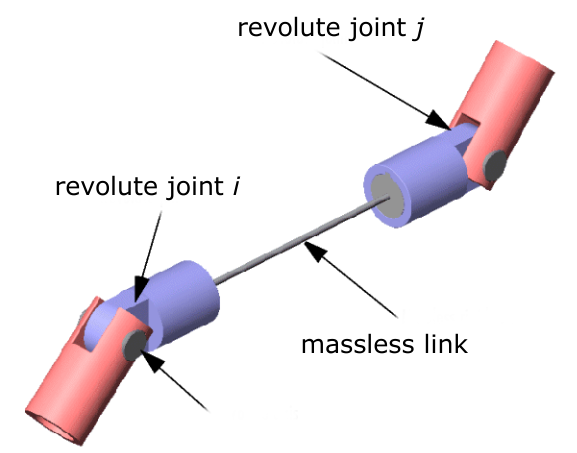
\includegraphics[width=0.5\linewidth]{images/kinematic_chains_1}
	\label{fig:kinematicchains1}
\end{figure}

\begin{figure}
	\centering
	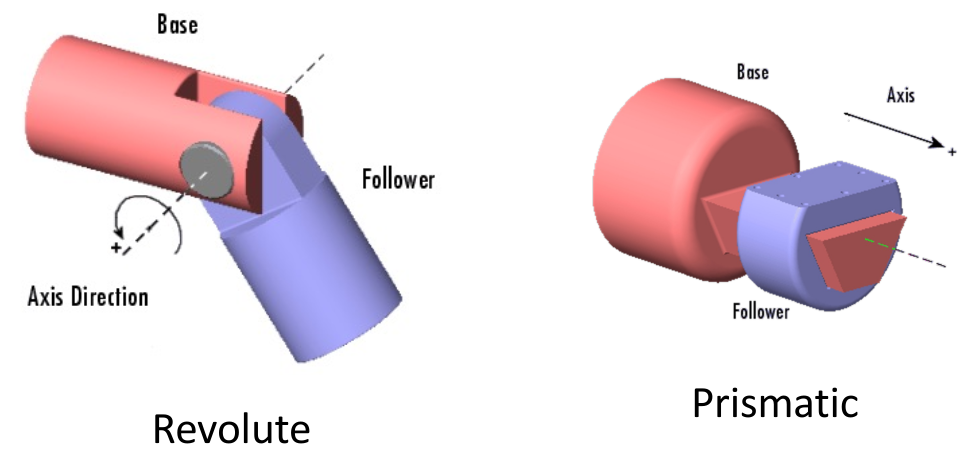
\includegraphics[width=0.6\linewidth]{images/kinematic_chains_2}
	\caption{Tipi di giunti}
	\label{fig:kinematicchains2}
\end{figure}

Noi analizzeremo solo \textbf{open chains} (in contrasto alle \textit{closed chains}): i.e. catene dove c'è solo 1 link fra due giunti qualunque. In questo caso la KC ha una struttura ad albero. Nel caso delle \textbf{closed chain}, invece, ci sono in generale più di un link fra due giunti e la struttura è ciclica.

I vari giunti sono schematizzati come mostrato in fig. \ref{fig:kinematicchains3}.

\begin{figure}[H]
	\begin{subfigure}{\linewidth}
		\centering
		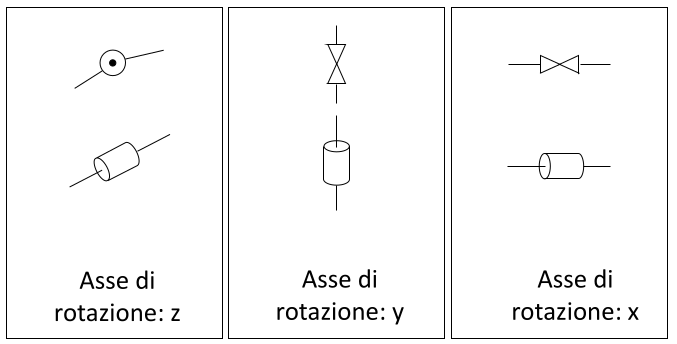
\includegraphics[width=0.6\linewidth]{images/kinematic_chains_3}
		\caption{Giunti rotoidali}
	\end{subfigure}
	\begin{subfigure}{\linewidth}
		\centering
		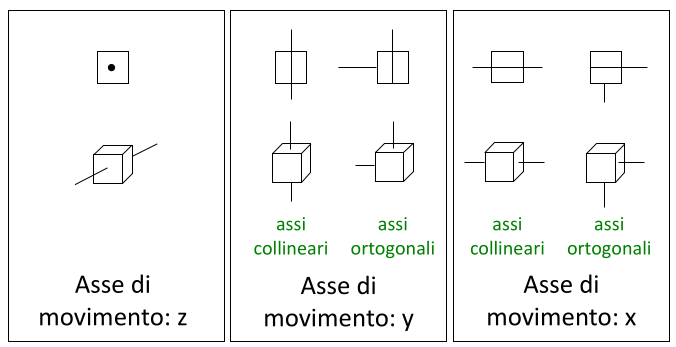
\includegraphics[width=0.6\linewidth]{images/kinematic_chains_4}
		\caption{Giunti prismatici}
	\end{subfigure}
	\caption{}
	\label{fig:kinematicchains3}
\end{figure}





\subsubsection{End Effector}

Oltre al braccio, un robot solitamente ha un \textit{tool} posto all'estremità (ultimo link). Questo è chiamato \textbf{end effector}, \textbf{gripper} o semplicemente \textbf{end tool}.

Il \textbf{TCP} (\textit{Tool Center Point}) è quel punto ideale sul'end-effector che i software muoveranno nello spazio. Come i vari giunti/link anche questo ha un proprio RF.

\begin{figure}
	\centering
	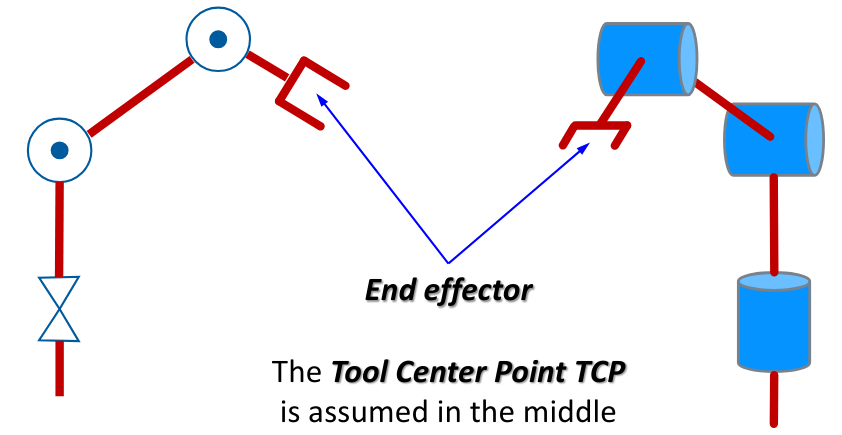
\includegraphics[width=0.6\linewidth]{images/kinematic_chains_5}
	\caption{Braccio robotico schematizzato}
	\label{fig:kinematicchains5}
\end{figure}



\section{Tipi di robot}

I robot industriali sono solitamente composti da una \textbf{shoulder} e un \textbf{wrist} (spalla e polso). Ponendo per notazione: P = "prismatic joint", R = "revolute joint". Di seguito i vari tipi, con le configurazioni delle relative shoulders.

\subsection{Possibili shoulder configurations}

\subsubsection{Cartesian}
\textbf{3P = P-P-P}: abbiamo 3 DoF, corrispondenti alle 3 coordinate cartesiane. Il \textit{task space} è un parallelepipedo. Posizionamento accurato ma desterità limitata.
\begin{figure}[H]
	\centering
	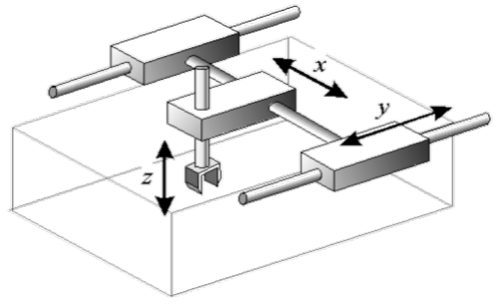
\includegraphics[width=0.35\linewidth]{images/kinematic_chains_6}
\end{figure}


\subsubsection{Cylindrical}	
\textbf{1R-2P = R-R-P}. Abbiamo 3 DoF, corrispondenti alle 3 coordinate cilindriche. Il \textit{task space} è una sezione di cilindro.\\
La stuttura essendo meno rigida rispetto al precedente ci da meno accuratezza (che va a diminuire con l'elongazione del braccio).

\begin{figure}[H]
	\begin{subfigure}{0.5\linewidth}
		\centering
		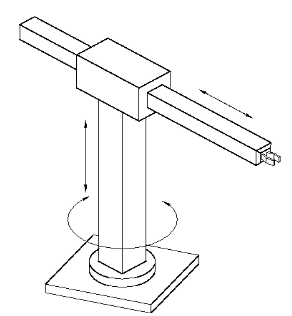
\includegraphics[width=0.4\linewidth]{images/kinematic_chains_7}
		\label{fig:kinematicchains7}
	\end{subfigure}
	\begin{subfigure}{0.5\linewidth}
		\centering
		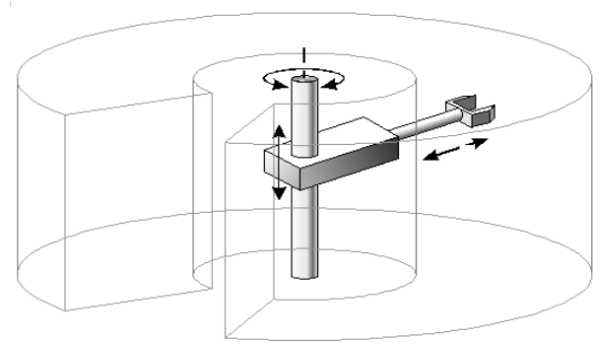
\includegraphics[width=0.65\linewidth]{images/kinematic_chains_16}
		\label{fig:kinematicchains16}
	\end{subfigure}
\end{figure}
	
\subsubsection{Polar or spherical}
\textbf{2R-1P = R-R-P}. Abbiamo 3 DoF, corrispondenti alle 3 coordinate polari. Il \textit{task space} è una sezione di una sfera. È ancora meno rigido rispetto alle precedenti (e come nel caso cilindrico l'accuratezza diminuisce con l'elongazione).
	
\begin{figure}[H]
	\centering
	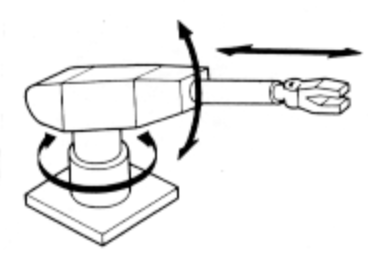
\includegraphics[width=0.25\linewidth]{images/kinematic_chains_10}
	\label{fig:kinematicchains10}
\end{figure}
	

\subsubsection{SCARA}
\textbf{2R-1P = R-R-P}. SCARA = Selective Compliance Assembly Robot Arm). Utili per manipolare piccoli componenti (e.g. $\mu$C). Abbiamo una corrispondenza fra DoM (degree of motion) e coordinata cartesiana solo per la componente verticale. L'effetto della gravità è compensato dalla struttura stessa, che è rigida verticalmente ma \textit{compliant} orizzontalmente.

\begin{figure}[H]
	\begin{subfigure}{0.5\linewidth}
		\centering
		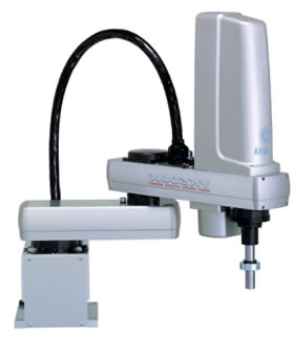
\includegraphics[width=0.4\linewidth]{images/kinematic_chains_8}
		\label{fig:kinematicchains8}
	\end{subfigure}
	\begin{subfigure}{0.5\linewidth}
		\centering
		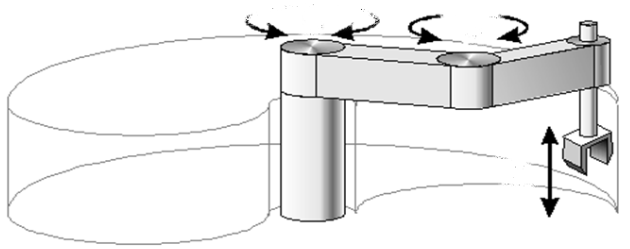
\includegraphics[width=0.7\linewidth]{images/kinematic_chains_15}
		\label{fig:kinematicchains15}
	\end{subfigure}
\end{figure}


\subsubsection{Articulated or Anthropomorphic}
\textbf{3R = R-R-R}. Simile ad un braccio umano. Non c'è corrispondenza fra giunti e coordinate cartesiane. Il \textit{task space} è una specie di sezione di una sfera. L'accuratezza non è costante in tutto il task-space. \textbf{È la tipologia più comune} visto che ci da la migliore desterità.

\begin{figure}[H]
	\centering
	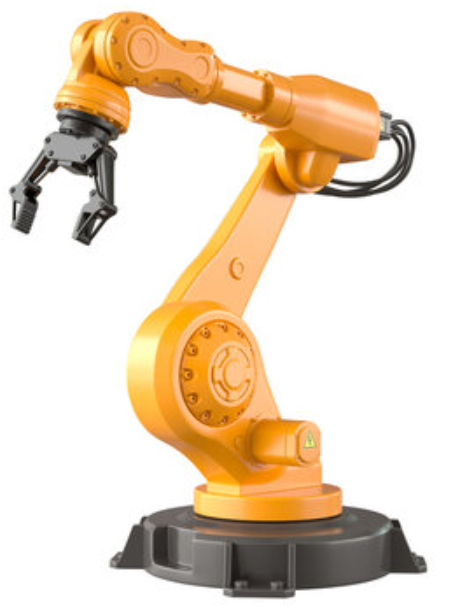
\includegraphics[width=0.15\linewidth]{images/kinematic_chains_9}
	\label{fig:kinematicchains9}
\end{figure}


\subsubsection{Parallel or closed chains}
Utili per manipolare payload pesanti, visto che questo tipo di struttura è molto rigida.

\begin{figure}[H]
	\begin{subfigure}{0.5\linewidth}
		\centering
		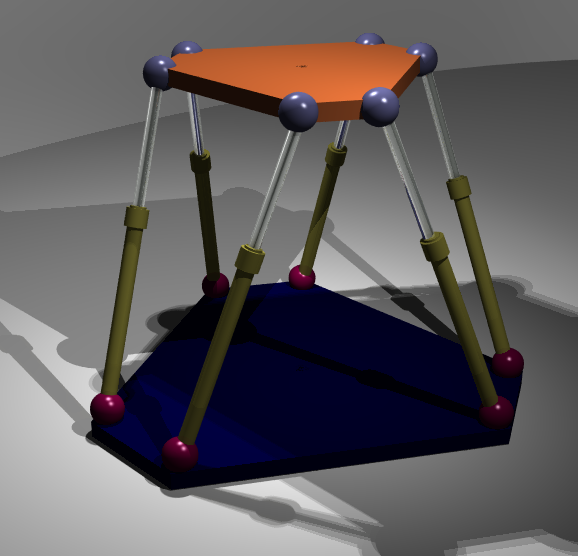
\includegraphics[width=0.3\linewidth]{images/kinematic_chains_11}
		\label{fig:kinematicchains11}
	\end{subfigure}
	 \hfill
	\begin{subfigure}{0.5\linewidth}
		\centering
		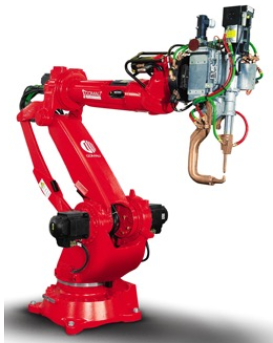
\includegraphics[width=0.3\linewidth]{images/kinematic_chains_12}
		\label{fig:kinematicchains12}
	\end{subfigure}
\end{figure}





\subsection{Wrist}
Lo scopo principale del polso è quello di orientare il TCP. Possiamo dire che la shoulder setta l'origine del TCP mentre il polso la sua orientazione.\\
La tipologia più comune è quello dello \textbf{spherical wrist}. Comunemente un wrist (sferico e non) è \textbf{composto da 3 rotational joints}.

\begin{figure}[H]
	\begin{subfigure}{0.6\linewidth}
		\centering
		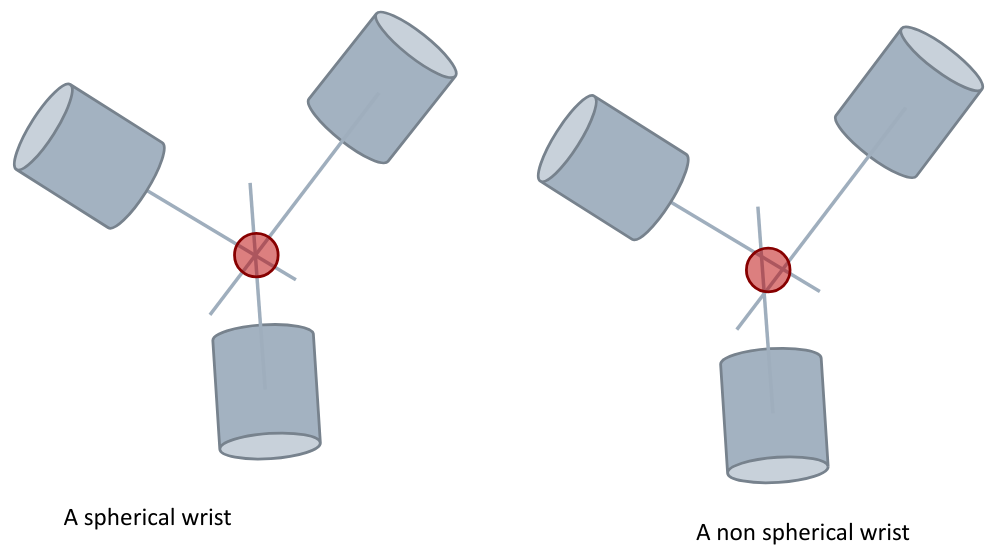
\includegraphics[width=0.8\linewidth]{images/kinematic_chains_13}
		\caption{Spherical vs non-spherical}
		\label{fig:kinematicchains13}
	\end{subfigure}
	\hfill
	\begin{subfigure}{0.4\linewidth}
		\centering
		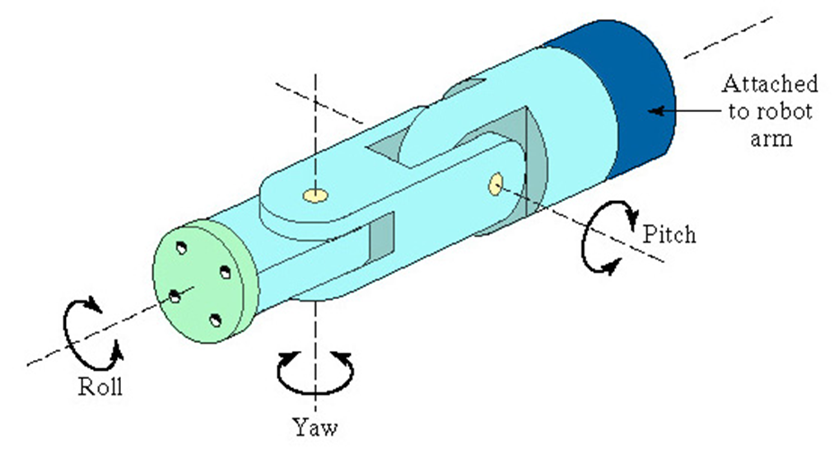
\includegraphics[width=0.9\linewidth]{images/kinematic_chains_14}
		\caption{Esempio}
		\label{fig:kinematicchains14}
	\end{subfigure}
\end{figure}





